S'ha dissenyat i construit dos prototips, anomenats TRITIUM-Aveiro i TRITIUM-IFIC-2, amb un disseny funcional i optimitzat per a la detecció del triti en els que tots els problems identificats en els dos primers prototips han sigut resolts. Aquests dos prototips, mostrats a la figura \ref{fig:PrototipsAveiroIFIC2}, presenten un disseny similar que consisteix en un atuell de PTFE a l'interior del qual se situen les fibres centellejadores. Per permetre la utilització d'un gran nombre de fibres (cents) aquestes es van situar lliurement dins l'atuell, prescindint de la matriu de PTFE i amb una densitat de fibres que permeta fluir l'aigua a través d'elles. A més, es van realitzar coincidències entre dos PMTs acoblats amb greix òptic a cada extrem de les fibres, necessari per a reduir el fons radioactiu tant com siga possible. Per poder realitzar de forma segura aquesta coincidència va ser necessari introduir a l'atuell dues finestres de polimetilmetacrilat (PMMA) que permeten als fotons generats a les fibres (dins de l'atuell) arribar fins als PMTs (fora del l'atuell). Els PMTs utilitzats en cada prototip són del model R$2154-02$ de Hamamtsu \cite{DataSheetPMTsAveiro} per a TRITIUM-Aveiro (el qual conté 360 fibres) i el model R$8520-406$ de Hamamatsu \cite{DataSheetPMTs} per a TRITIUM-IFIC-2 (el qual conté 800 fibres). Aquests dos prototips presenten diferències subtils en el disseny. Entre les més importants es troben:
\begin{enumerate}
\item{} El diàmetre de les fibres, $2~\mm$ per a les utilitzades en TRITIUM-Aveiro i $1~\mm$ per a les utilitzades en TRITIUM-IFIC-2. Un diàmetre més gran li confereix una major rigidesa al prototip i millora el flux de l'aigua a través de les fibres. No obstant això, també implica una relació senyal/fons menor, donant lloc a una eficiència més baixa i, per tant, a una MDA per al triti més alta.
\item{} A més, el protocol de tractament de la superfície de les fibres centellejadores no va ser aplicat a les fibres utilitzades en TRITIUM-Aveiro ja que aquest encara no estava desenvolupat. Com s'ha provat amb tests experimentals, aquest tractament millora la intensitat del senyal en més d'un factor dos, que a causa dels xicotets senyals generats pels esdeveniments del triti implica una millora substancial en l'eficiència de detecció.
\item{} L'ús de fotosensors diferents. TRITIUM-Aveiro utilitza dos PMTs en coincidència mentre que la proposta per a TRITIUM-IFIC-2 és utilitzar matrius de SiPMs. Els SiPMs tenen una major eficiència de fotodetecció, que dona com a resultat una major eficiència de la detecció del triti. No obstant això, aquests presenten un soroll electrònic més alt, incrementant el fons mesurat pel detector. %Cal tenir en compte que aquesta serà una diferència per al futur ja que, fins ara, les mesures han estat preses sols amb PMTs. 
\end{enumerate} 
Totes aquestes opcions seran provades i aquelles amb millors resultats seran implementades al prototip final.
\begin{figure}
\centering
    \begin{subfigure}[b]{0.5\textwidth}
    \centering
    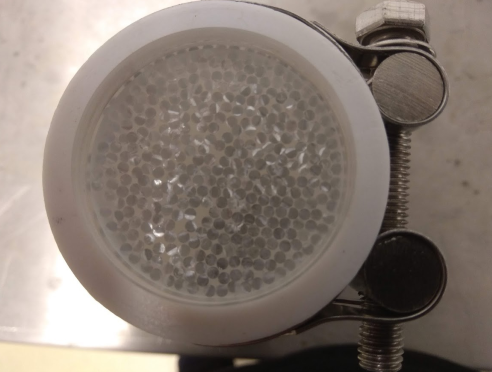
\includegraphics[width=\textwidth]{12Summary/5Prototypes/53FinalPrototypes/531TritiumAveiro/TeflonVessel_Fibers.png}  
        \caption{}\label{subfig:PrototipAveiro}
    \end{subfigure}
    \hfill
    \begin{subfigure}[b]{0.5\textwidth}
    \centering
    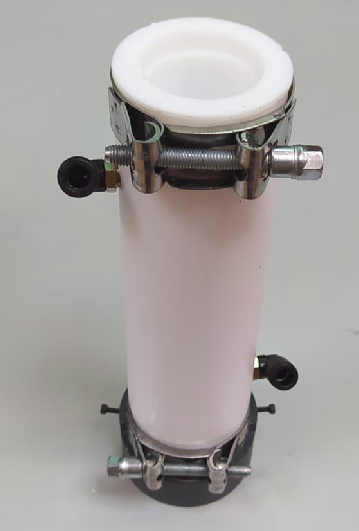
\includegraphics[width=\textwidth]{12Summary/5Prototypes/53FinalPrototypes/532TritiumIFIC2/Tritium_IFIC_2_vessel1.png}  
    \caption{\label{subfig:PrototipIFIC2}}
    \end{subfigure}
\caption{a) Atuell de TRITIUM-Aveiro. b) Atuell de TRITIUM-IFIC-2. \label{fig:PrototipsAveiroIFIC2}.}
\end{figure}
L'objectiu d'aquests prototips és mesurar l'eficiència de la detecció del triti i la MDA. Per tant, l'activitat de la dissolució d'aigua tritiada emprada va ser $30$ i $10~\kilo\becquerel/\liter$ per a TRITIUM-Aveiro i TRITIUM-IFIC-2, respectivament. Aquesta activitat es inferior a la utilitzada en els prototips inicials.

Els espectres d'energia mesurats amb TRITIUM-IFIC-2 i les respectives taxes de comptatge mesurades són  mostrades a la Figura \ref{fig:EspectresEnergeticsTRITIUMIFIC2} i a la Taula \ref{tab:ContesPerSegonTRITIUMIFIC2}, respectivament. TRITIUM-Aveiro utilitza una electrònica diferent que mesura directament taxes de comptatge sense la necessitat d'obtenir els espectres d'energia. Aquestes taxes obtingudes són també mostrades a la Taula \ref{tab:ContesPerSegonTRITIUMIFIC2}.

\begin{figure}
\centering
    \begin{subfigure}[b]{1\textwidth}
    \centering
    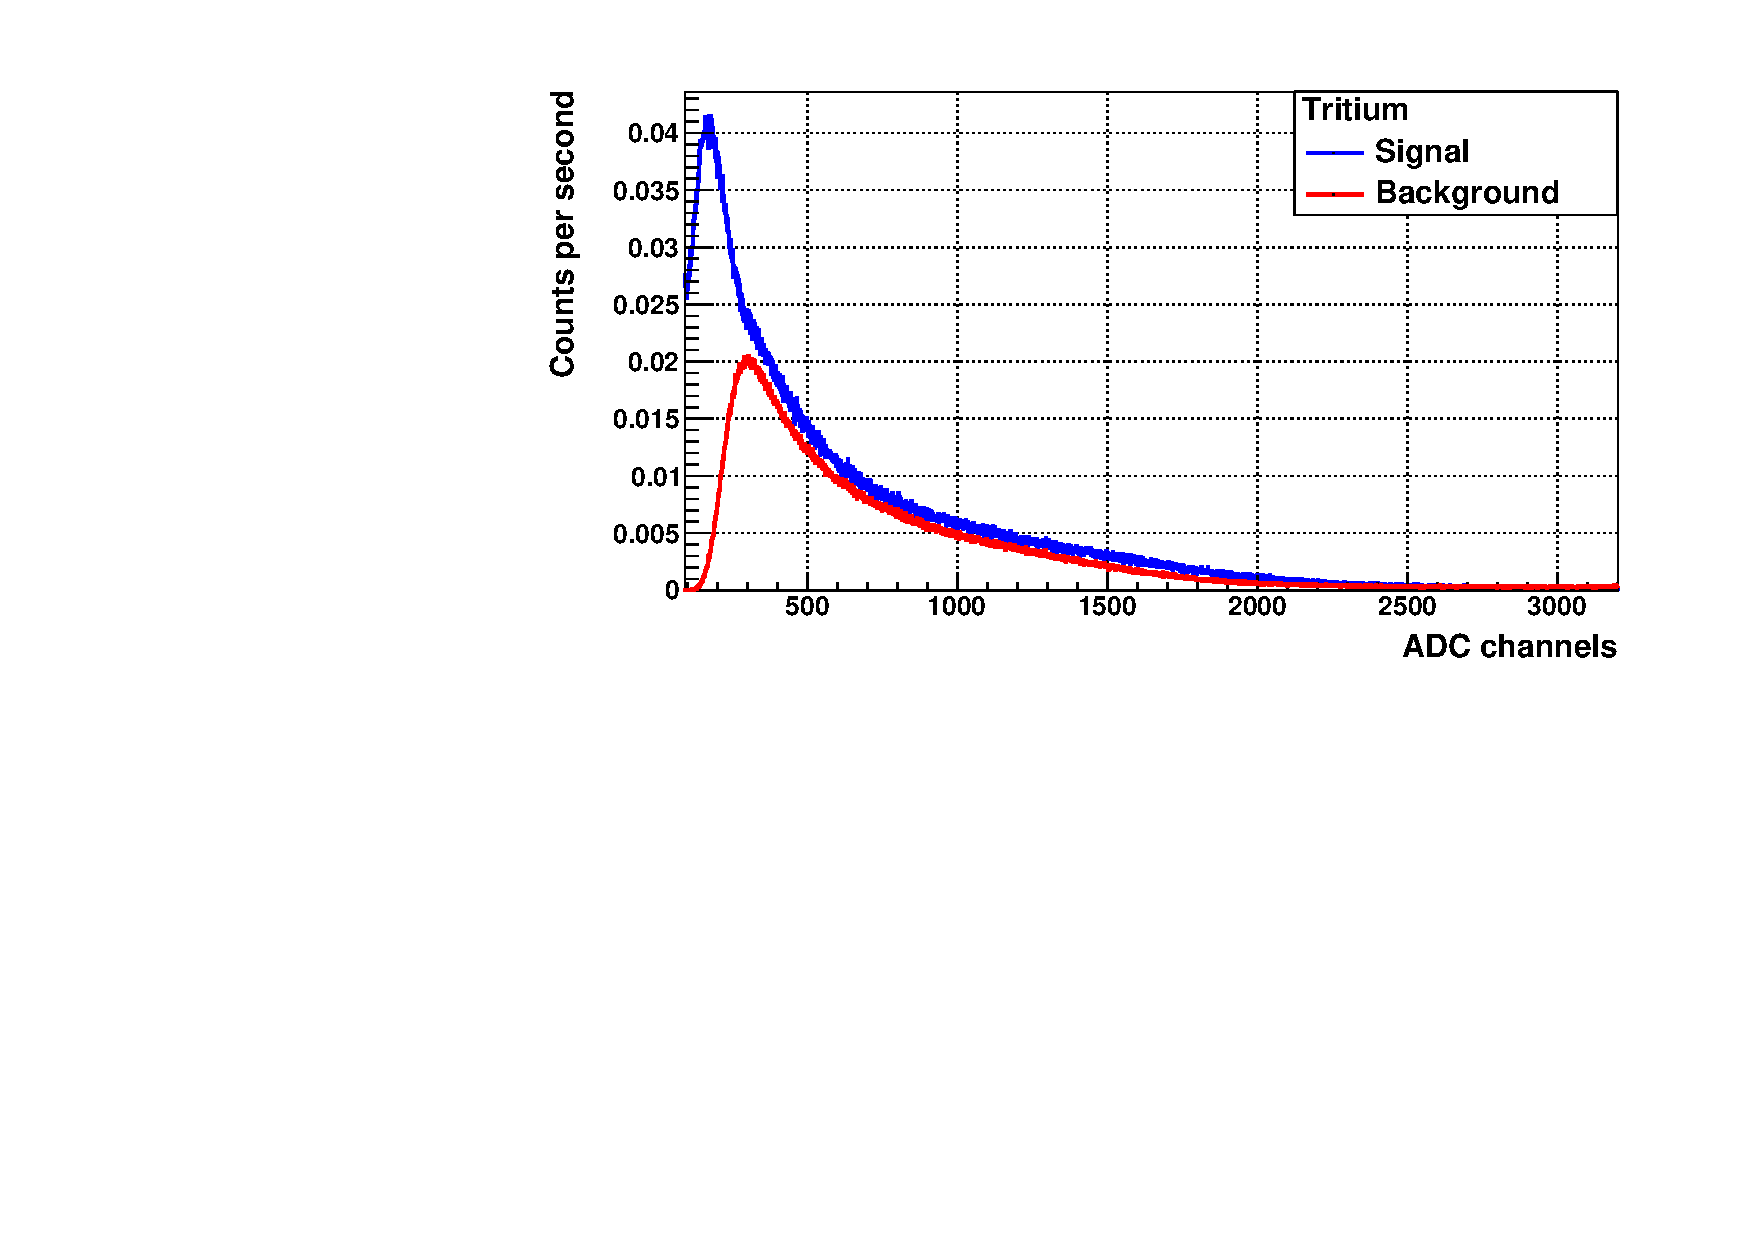
\includegraphics[width=\textwidth]{12Summary/5Prototypes/53FinalPrototypes/532TritiumIFIC2/TritiumIFIC2SignalsHigherZOOM_NP.pdf}  
    \caption{\label{subfig:EspectreEnergeticSenyalFonsTritiumIFIC2}}
    \end{subfigure}
    \hfill
    \begin{subfigure}[b]{1\textwidth}
    \centering
    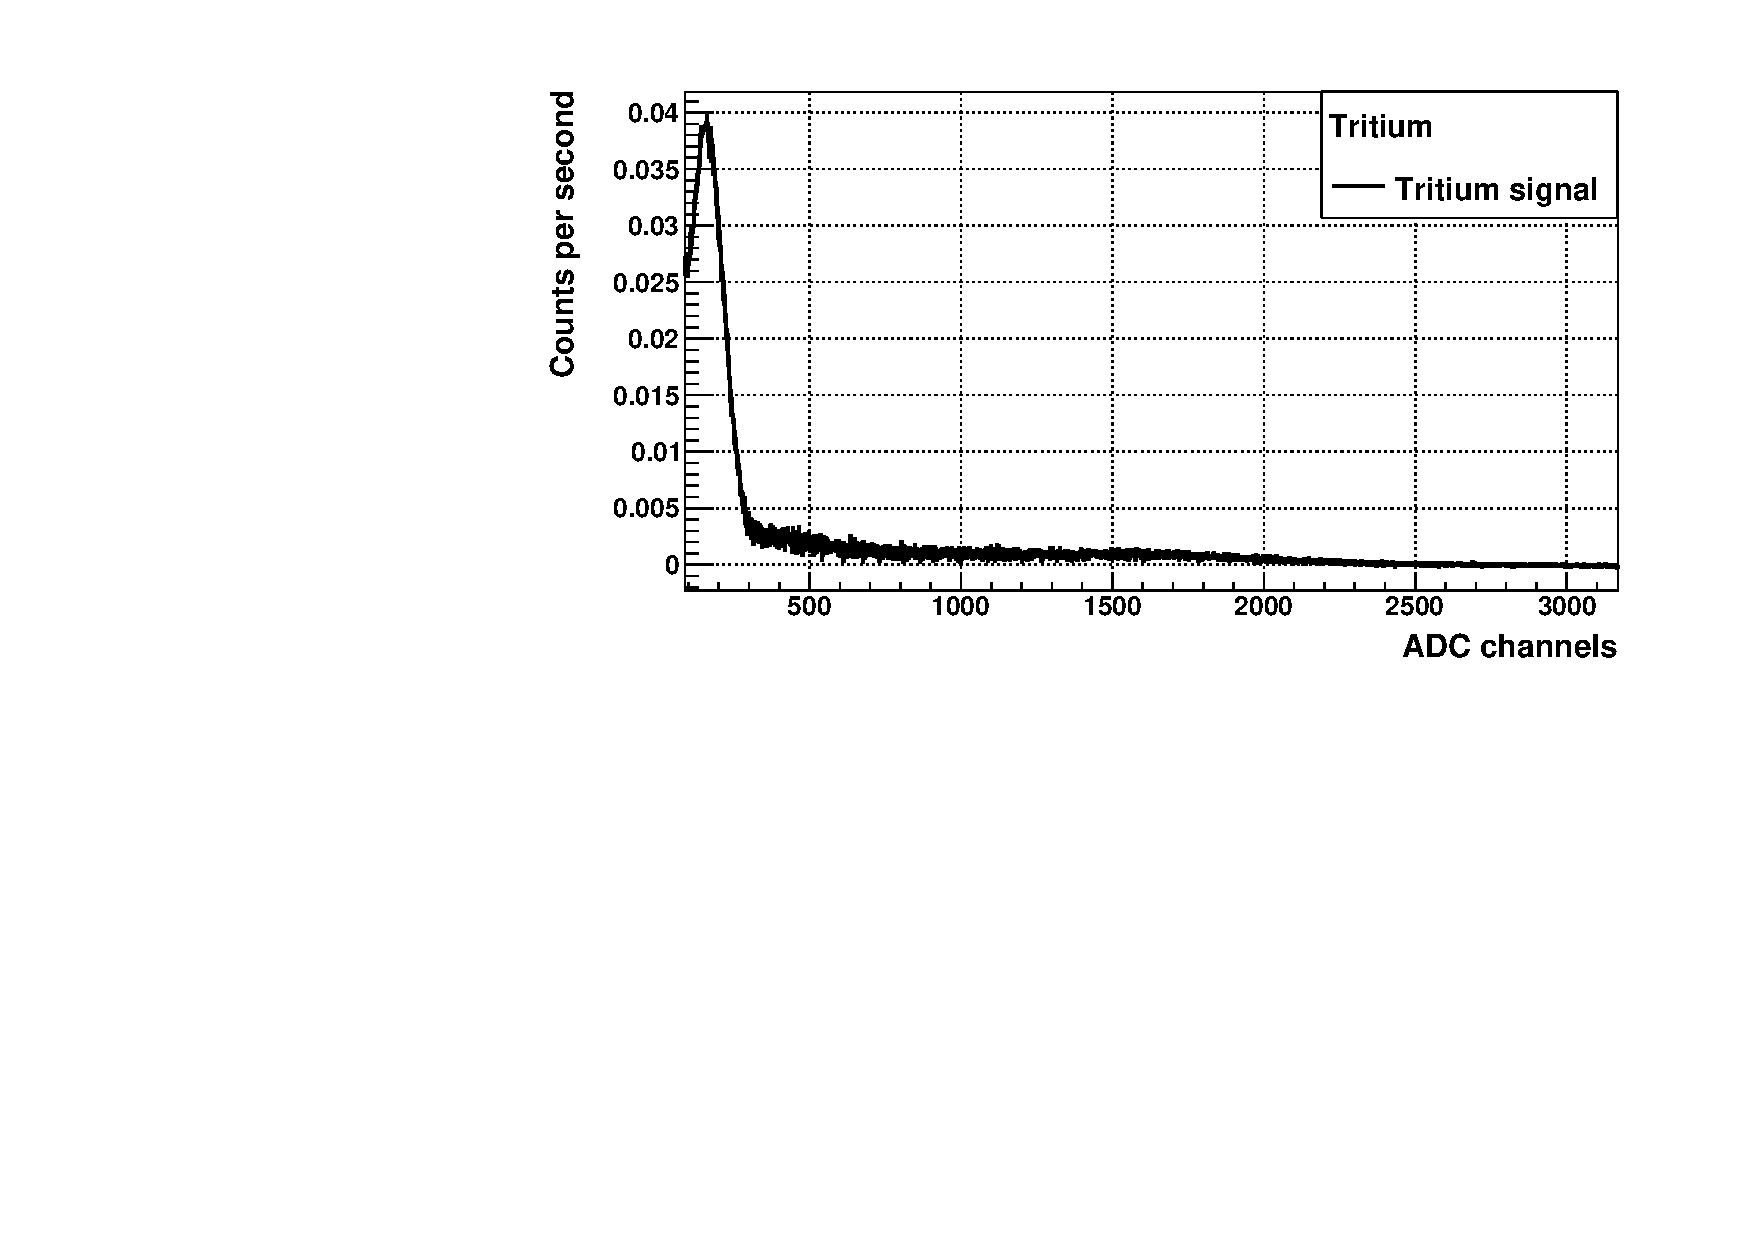
\includegraphics[width=\textwidth]{12Summary/5Prototypes/53FinalPrototypes/532TritiumIFIC2/TritiumIFIC2ClearHigherZOOM_NP.pdf}  
    \caption{\label{subfig:EspectreEnergeticTritiTritiumIFIC2}}
    \end{subfigure}
 \caption{Espectres d'energia mesurats amb TRITIUM-IFIC-2. a) Espectre d'energia de senyal i fons. b) Espectre d'energia del triti.}
 \label{fig:EspectresEnergeticsTRITIUMIFIC2}
\end{figure}

\begin{table}[htbp]
\centering{}%
\begin{tabular}{ccc}
\toprule 
Espectres & TRITIUM-Aveiro & TRITIUM-IFIC-2  \tabularnewline
\midrule
\midrule 
Prototip del senyal & $10,9 \pm 0,4$ & $19,05 \pm 0,18$ \tabularnewline
Prototip del fons & $9,0 \pm 0,4$ & $11,54 \pm 0,14$ \tabularnewline  
Espectre de triti & $1,9 \pm 0,6$ & $7,11 \pm 0,23$ \tabularnewline
\bottomrule
\end{tabular}
\caption{Taxes de comptatge mesurades amb el prototip TRITIUM-IFIC-2.}
\label{tab:ContesPerSegonTRITIUMIFIC2}
\end{table}

L'eficiència específica de la detecció del triti en agua es
$$S = (1,6 \pm 0,5)\cdot{} 10^{-5}~\liter\:\kilo\becquerel^{-1}\second^{-1}\cm^{-2}$$
$$S = (14,1 \pm 0,6)\cdot{} 10^{-5}~\liter\:\kilo\becquerel^{-1}\second^{-1}\cm^{-2}$$
per a TRITIUM-Aveiro i TRITIUM-IFIC-2, respectivament. Com es pot observar l'eficiència de TRITIUM-IFIC-2 millora l'obtinguda amb els prototips anteriors i els detectors de triti similars desenvolupats fins ara \cite{Hofstetter1, Hofstetter2}. Veiem per tant que s'ha superat l'estat actual de l'art de la detecció de triti en l'aigua utilitzant plàstics centellejadors. No obstant això, trobem una eficiència específica inferior a l'esperada per al prototip TRITIUM-Aveiro. Tot indica que aquest dèficit d'eficiència és causat principalment per l'absència del tractament de la superfície a les fibres centellejadores, una cosa que ha de ser estudiat amb més deteniment.

La mínima activitat de triti mesurable pels prototips s'obté aplicant el criteri de Currie \cite{Knoll}. Els valors obtinguts són $3,6$ i $0,2~\kilo\becquerel/\liter$ per a mesures d'una hora per a TRITIUM-Aveiro i TRITIUM-IFIC-2, respectivament. 

L'estabilitat de l'eficiència del prototip TRITIUM-IFIC-2 es va comprovar fent mesures al llarg de mesos, les quals es mostren a la Figura \ref{fig:MonitoritzacioTRITIUMIFIC2}. Com es pot observar, no s'aprecia cap decreixement durant els sis mesos de mesura, obtenint-se un comportament estable del detector amb una desviació estàndard relativa de la taxa de comptatge del $2,5\%$.

\begin{figure}[h]
\centering
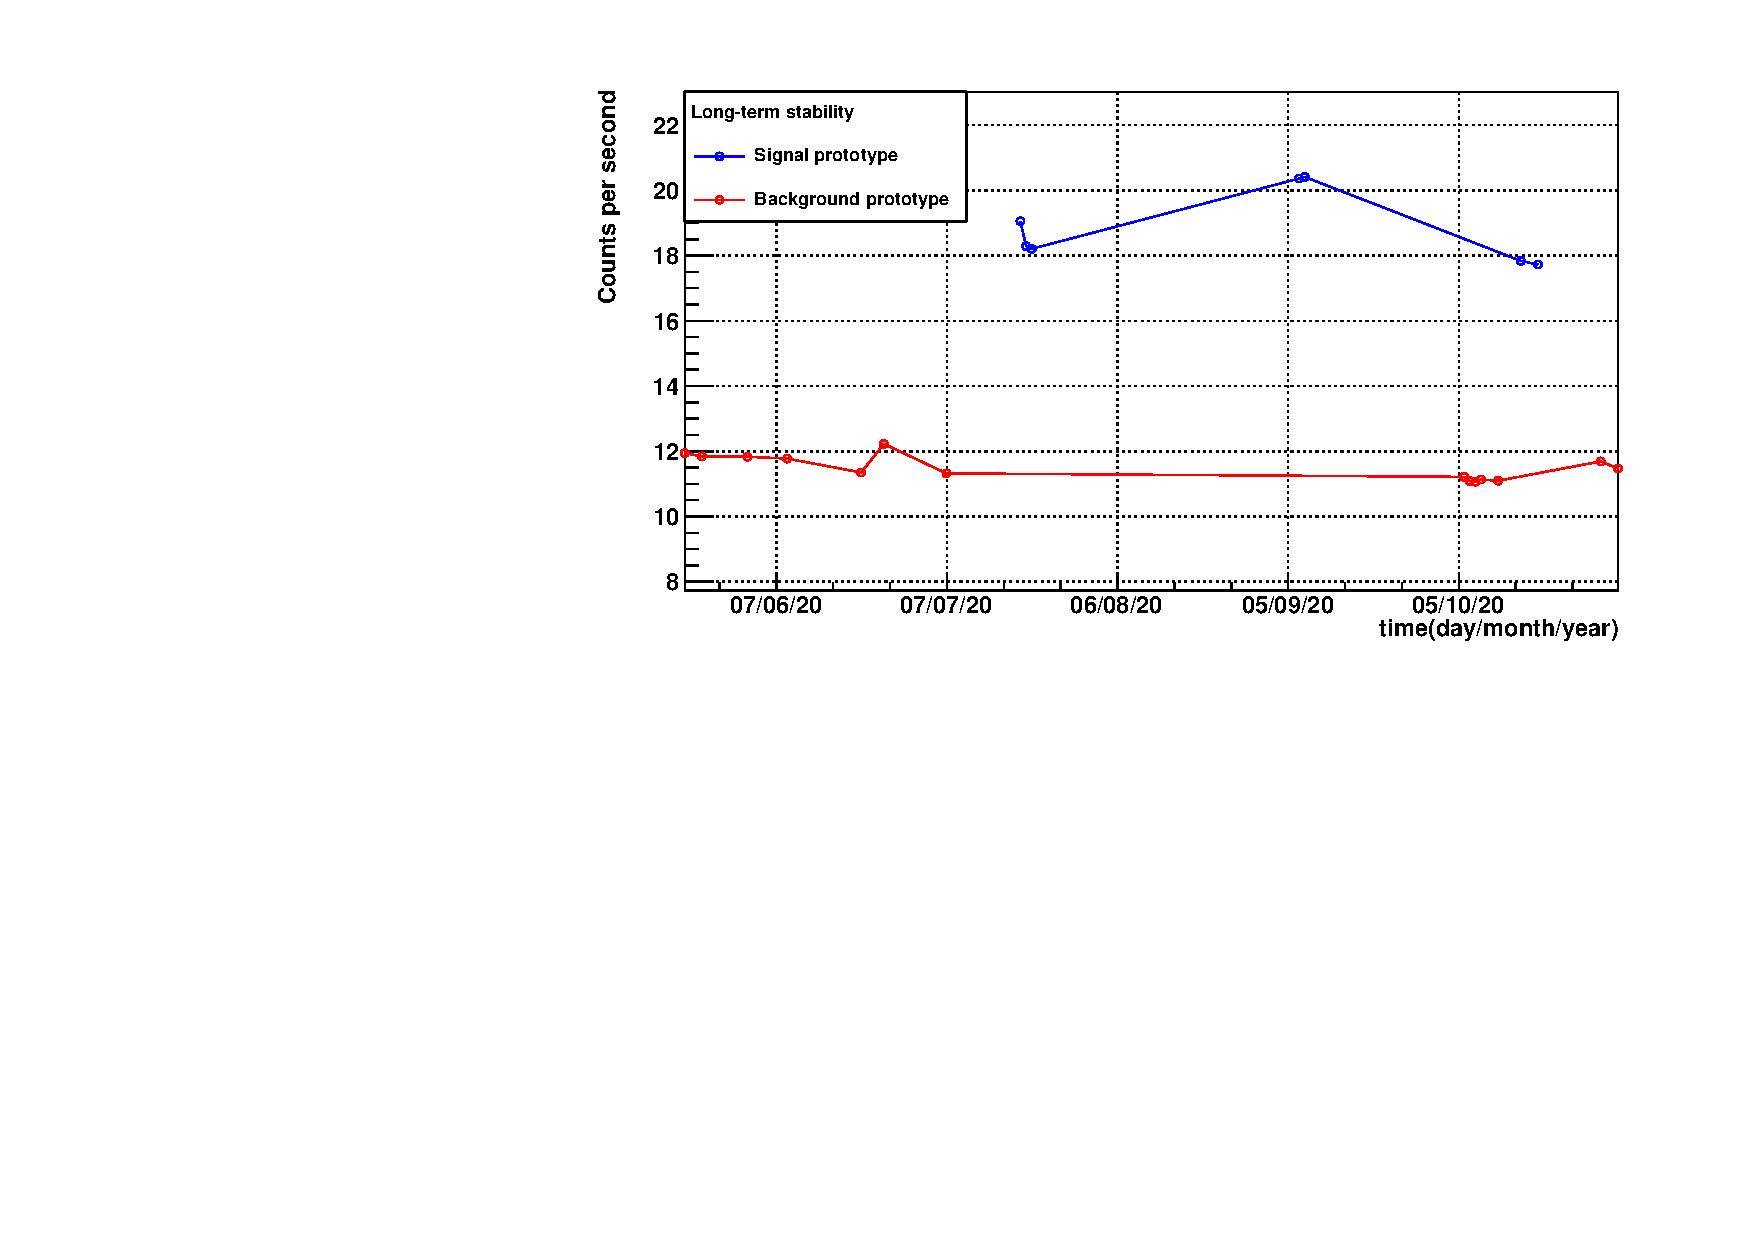
\includegraphics[scale=0.7]{12Summary/5Prototypes/53FinalPrototypes/532TritiumIFIC2/Signal_Background_stability_ZOOM.pdf}
\caption{Taxes de comptatge de fons i senyal mesurades amb el prototip TRITIUM-IFIC-2 al llarg de diversos mesos.\label{fig:MonitoritzacioTRITIUMIFIC2}}
\end{figure}

El prototip TRITIUM-Aveiro va ser instal·lar en Arrocampo el 27 de març de 2019 i va estar prenent mesures del fons radioactiu durant més de quatre mesos, fins al 18 d'agost de 2019. En aquestes mesures, mostrades a la Figura \ref{fig:FonsArrocampoAveiro}, es pot observar una gran estabilitat al voltant d'una taxa de comptatge de $9,31$. També s'observa un pic el dia 2 de maig causat per l'obertura del castell de plom.

\begin{figure}[h]
\centering
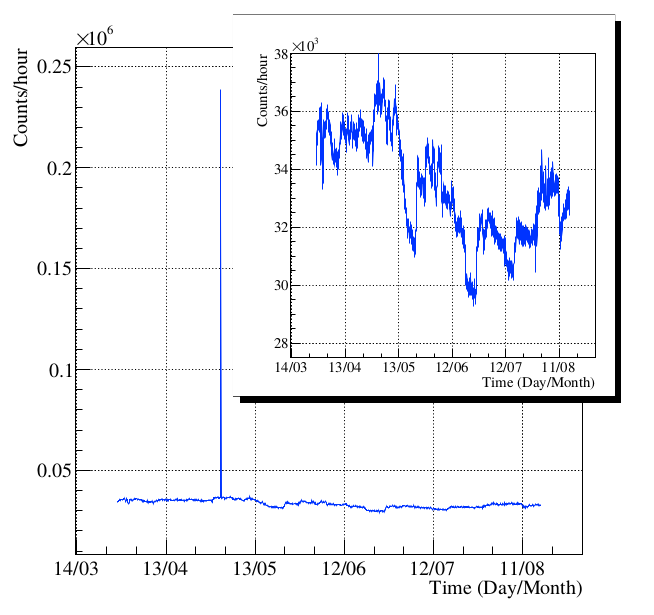
\includegraphics[scale=0.45]{12Summary/5Prototypes/54ArrocampoMeasurements/721TRITIUMAVEIRO0/BackgroundMeasurements.png}
\caption{Mesures del fons radioactiu d'Arrocampo obtingudes amb el prototip TRITIUM-Aveiro.\cite{ExperimentalPaperCarlos}.\label{fig:FonsArrocampoAveiro}}
\end{figure}